\documentclass[11pt]{exam}
\usepackage[margin=1in]{geometry}
\pagestyle{plain}
\usepackage{amsmath,amsfonts,amssymb,amsthm,enumerate}
\usepackage{multicol}
\usepackage[]{graphicx}
\usepackage{hyperref}
\usepackage{tikz}
\usepackage{pgfplots}
\usepackage{subfigure}
\usepackage[final]{pdfpages}

\addtolength{\footskip}{2\baselineskip} % to lower the page numbers
\title{\vspace{-0.5in} Math 115 \\ Worksheet Section 2.4}
\date{}


% \theoremstyle{definition}
% \newtheorem{problem}{Problem}
\renewcommand{\questionlabel}{\textbf{Problem~\thequestion.}}
%\printanswers

\begin{document}
\maketitle
\vspace{-0.75in}
\begin{questions}
%
% Let them try this one first!  Given them about 5 minutes to work in groups at the board.  Most of them will struggle and give sentences where "per year" is involved in some way.  That's ok!  Once they've all thought on it a bit, have them sit down and finish it up together.  But it is KEY to have them try it first so they are receptive to how hard this is and what they need to look for!
%
% You probably want to start with an interpretation about what happens when the interest rate goes from 5% to 6%, to avoid additional complexity.  But then point out that 1% is actually a very large jump given the context, and ask them complete a sentence that you begin "If the interest rate decreases from 5% to 4.9%, then...."  Students catch on to this quickly.  That doesn't mean these problems are easy!  Students struggle to get to the point where they understand intuitively what the derivative is telling them in the first place.
%
%
  \question Investing \$1000 at an annual interest rate of $r$\%, compounded continuously, for 10 years gives you a balance of \$$B$, where $B=g(r)$.  
\begin{enumerate}
	\item Give a practical interpretation of $g(5)=1649$.
	\item What are the units on $g'(5)$?
	\item Give a practical interpretation of $g'(5)=165$.
\end{enumerate}
\begin{solution}
  \begin{enumerate}
  \item Investing \$1000 at an annual 5\% interest rate, compounded continuously, for \(10\) years
    will give a balance of \(\$1649\).
  \item \(\$/\%\)
  \item If the interest rate increases from \(5\%\) to \(5.1\%\), then
    the projected balance after \(10\) years increases by
    approximately \(\$16.50\).
  \end{enumerate}
\end{solution}
\pagebreak
\question Suppose that the revenue, in dollars, of the manufacturer of
  a certain chemical is $R(q)=100q-2q^3$, where $q$ is the quantity of
  the chemical sold, in kilograms. We estimate $R'(2)=76$.
  Interpret this practically.
  \begin{solution}
   If the quantity of the chemical sold is increased from \(2\)kg to
   \(2.1\)kg, then the revenue will increase by approximately \(\$7.60\).
  \end{solution}
\question (2.4 \#3) The temperature, $T$, in degrees Fahrenheit, of a cold yam placed in a hot oven is given by $T=f(t)$, where $t$ is the time in minutes since the yam was put in the oven.
\begin{enumerate}
\item What is the sign of $f'(t)$?  Why?
\vskip2ex


\item What are the units of $f'(20)$?

\vskip2ex

\item The following answers were given as practical interpretations of $f'(20)=2$.  Evaluate each one and correct if necessary.
\begin{enumerate}


%no direction, no approximate
\item After the yam has been in the oven for 20 minutes, its temperature will change by $2^\circ$F in the next minute.

\vskip2ex
%good
%\item During its 21st minute in the oven, the temperature of the yam increases by approximately $2^\circ$F.
%\vskip2ex

%not local
\item After the yam has been in the oven for 20 minutes, the yam's temperature will rise by about $2^\circ$F each additional minute.
\vskip2ex

%no  "rates" allowed
\item During its 21st minute in the oven, the temperature of the yam is increasing at about $2^\circ$F per minute.

\vskip2ex

%didn't convert rates correctly
\item  After the yam has been in the oven for 20 minutes, the yam's temperature will increase by about $0.2^\circ$F if it stays in the oven an additional 10 seconds.
\vskip2ex

%too wide
\item The yam's temperature will increase by about $4^\circ$F between minutes 18 and 20 of being in the oven.

\vskip2ex

\end{enumerate}
\end{enumerate}
\begin{solution}
  \begin{enumerate}
  \item The sign is positive since the yam is getting hotter.
  \item \({}^\circ\)F/minute
  \item Corrections
    \begin{enumerate}
\item After the yam has been in the oven for 20 minutes, its
  temperature will \textbf{increase} by \textbf{approximately} $2^\circ$F in the next minute.

\vskip2ex
%good
%\item During its 21st minute in the oven, the temperature of the yam increases by approximately $2^\circ$F.
%\vskip2ex

%not local
\item After the yam has been in the oven for 20 minutes, the yam's
  temperature will rise by about $2^\circ$F \textbf{in the next minute}.
\vskip2ex

%no  "rates" allowed
\item During its 21st minute in the oven, the temperature of the yam
  \textbf{will increase by about $2^\circ$F in the next minute.}

\vskip2ex

%didn't convert rates correctly
\item  After the yam has been in the oven for 20 minutes, the yam's temperature will increase by about $0.2^\circ$F if it stays in the oven an additional \textbf{6} seconds.
\vskip2ex

%too wide
\item The yam's temperature will increase by about $\mathbf{2}^\circ$F between minutes \textbf{19} and 20 of being in the oven.
    \end{enumerate}
  \end{enumerate}
\end{solution}
\question  Let $f(t)$ be the number of centimeters of rainfall that has
fallen since midnight, where $t$ is the time in hours. Interpret
the following in practical terms, giving units.

\begin{enumerate}
\item $f(10)=2.1$

\vfill
\item $f^{-1}(5)=16$

\vfill
\item $f'(10)=0.4$

\vfill
\item $(f^{-1})'(5)=2$

  \begin{solution}
    \begin{enumerate}
    \item \(2.1\)cm of rainfall has occurred from midnight to 10am.
    \item \(5\)cm of rainfall has occurred from midnight to 4pm.
    \item From \(10\)am to \(11\)am, approximately \(0.4\)cm of
      rainfall will occur.
    \item To answer this problem, first consider that \(f^{-1}\) is a
      function taking rainfall since midnight to hours after
      midnight. Thus, if \(R\) is rainfall, this is saying the relationship between \(\Delta
      R\) and \(\Delta t\) after \(5\) inches of rainfall is given by \(\frac{\Delta t}{\Delta R} = 5 \implies
      \Delta t = 2 \Delta R\). Thus, our answer is ``After 5 inches of
      rainfall, approximately another 2 inches of rainfall will occur
      in the next hour.''
    \end{enumerate}
  \end{solution}

%
% Instructor note: they will often mix up f inverse prime, with f prime inverse.  Tell them to think about f inverse as just some function g, and they want to interpret g', just like they've been doing.  What remains is just to figure out the appropriate units for the various quantities.
%

\vfill
\end{enumerate}
\question  Suppose $g(v)$ is the fuel efficiency, in
miles per gallon (mpg), of a van going at a speed of $v$ miles per hour. Complete the sentence to give a practical interpretation of
 $(g^{-1})'(20)=-2$.
 
 \vskip1ex
 \textit{To have a fuel efficiency of 20 mpg instead of 18 mpg, the driver should...}
 \vfill
 \begin{solution}
   Consider that we have change in speed over change in fuel efficiency is approximately \(-2\)
   mph/mpg at \(20\) mpg, that is \(\frac{\Delta v}{\Delta g} \approx
   -2\) at \(20\) mpg. So, increasing fuel efficiency by 1mpg would
   require a decrease in speed by 2mph. Thus, if \(\Delta g = 2\), we
   get that we need \(\Delta v \approx -2 \cdot \Delta g = 4\) mph. Thus, 
   to have a fuel efficiency of 20 mpg instead of 18 mpg, the driver
   should drive approximately 4 mph slower.
 \end{solution}
\textit{Extra practice}:  2.4 \#1--10, 13, 19, 21, 31, 33, 37, 39, 43, 47, 64--65.  \textbf{\underline{Practice this}.}  Also note that answers in the back of the book may \textbf{not} satisfy the requirements we discussed.
\pagebreak
\question (Fall 2015 Exam 1) Algernon Brayik is making scones. He knows that the height of a scone is a function of how much baking soda it contains. Let h(B) be the height in millimeters of a scone that contains B grams of baking soda. Assume that the function h is increasing and invertible, and that h and h-1 are both differentiable.
\begin{enumerate}[(a)]
	\item Algie looks in his baking soda container and finds that there are exactly 46 grams of baking soda remaining. Suppose he uses all of this baking soda to make 8 scones, and that the baking soda is equally distributed among all 8 of the scones. Write a mathematical expression involving h or $h^{-1}$ for the height (in millimeters) of each resulting scone.
	\item Below is the first part of a sentence that will give a practical interpretation of the equation $h'(6) = 15$ in the context of this problem. Complete the sentence so that the practical interpretation can be understood by someone who knows no calculus. Be sure to include units in your answer.
	
	\emph{If Algie decreases the amount of baking soda per scone from 6 grams to 5.8 grams, then...}
	
	Algie makes a batch of scones, with each scone containing k grams of baking soda (for some constant k). When the scones come out of the oven, he decides they are each 10 millimeters shorter than he would like. Write a mathematical expression involving $k$, $h$, and $h^{-1}$ for the number of grams of baking soda per scone he should use to get scones of the desired height.
	
	\item Algie does some calculations and determines that $\displaystyle\frac{60}{h^{-1}(30)}=40$.
	Based on this information, which of the following statements must be true?
Circle all of the statements that must be true or circle none of these.
\begin{enumerate}[A.]
\item If Algie makes 40 scones, each with 30 grams of baking soda, then the scones will rise to a height of 60 millimeters.
\item If Algie wants to make 40 scones, then he must use 60 grams of baking soda.
\item If Algie wants to make scones of height 30 millimeters and he has 60 grams of baking soda, then the maximum number of scones he can make is 40.
\item A scone containing 1.5 grams of baking soda rises to a height of 30 millimeters.
\item A scone containing 30 grams of baking soda rises to a height of 1.5 millimeters.
\item None of these
\end{enumerate}
\end{enumerate}
\begin{solution}
  See \href{https://dhsp.math.lsa.umich.edu/exams/115exam1/f15/s4.pdf}{https://dhsp.math.lsa.umich.edu/exams/115exam1/f15/s4.pdf}
\end{solution}
\question (Winter 2010 Exam 1) Suppose that $W(h)$ is an invertible function which tells us how many gallons of water an oak tree of height $h$ feet uses on a hot summer day.
	
\begin{enumerate}[(a)]	
\item Give a practical interpretations for each of the following quantities or statements that can be understood by someone who knows no calculus. Be sure to include units in your answer.
\begin{multicols}{3}
	\begin{enumerate}[(i)]
		\item $W(50)$.
		\item $W^{-1}(40)$.
		\item $W'(5)$.
	\end{enumerate}
\end{multicols}	
	\item Suppose that an average oak tree is A feet tall and uses G gallons of water on a hot summer day. Answer each of the questions below in terms of the function W. You may also use the constants A and/or G in your answers.
\begin{enumerate}[(i)]
	\item A farmer has a grove with 25 oak trees, and each one is 10 feet taller than an average oak tree. How much water will be used by his trees during a hot summer day?
	\item The farmer also has some oak trees which each use 5 fewer gallons of water on a hot summer day than an average oak tree does. How tall is one of these trees?
\end{enumerate}

\end{enumerate}
\begin{solution}
 See \href{https://dhsp.math.lsa.umich.edu/exams/115exam1/w10/s9.pdf}{https://dhsp.math.lsa.umich.edu/exams/115exam1/w10/s9.pdf}
\end{solution}
\question (Fall 2011 Exam 1) The Twitter Celebrity Index (TCI) measures the celebrity of Twitter users; the function T(x) takes the number of followers (in millions) of a given user and returns a TCI value from 0 to 10. Below is a graph of this function.
	\begin{figure}[h]
		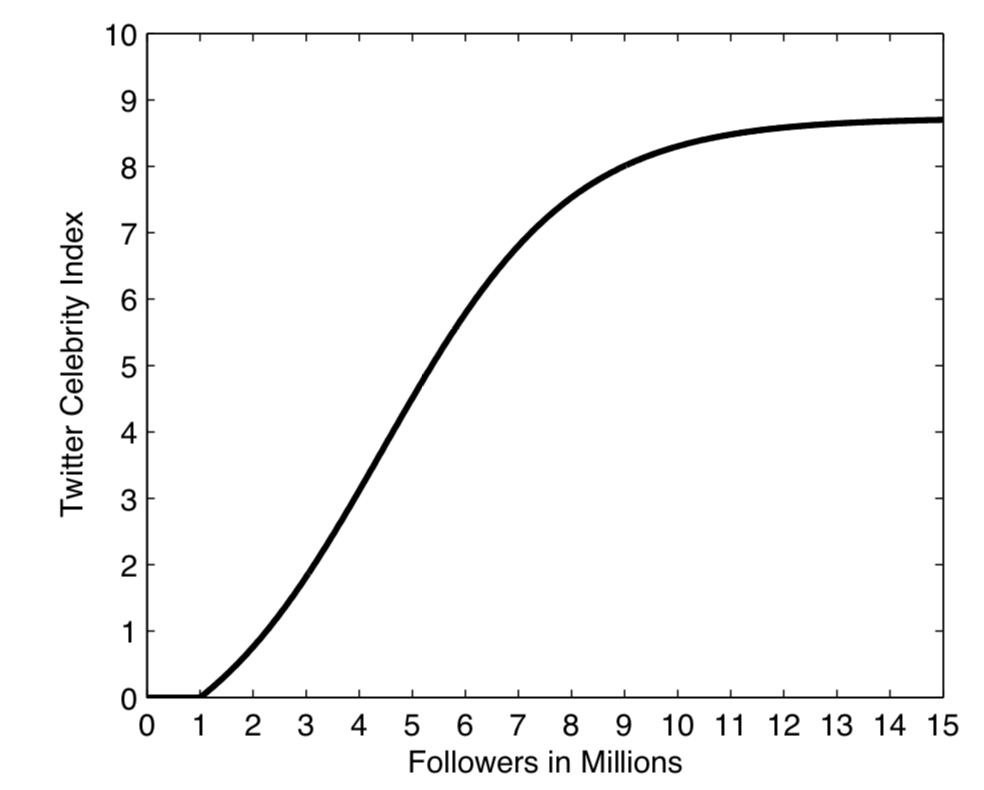
\includegraphics[scale=0.4]{Twitter.png}
	\end{figure}
Use the graph above to help you answer the following questions. Give a practical interpretation of each equation in the context of this problem that can be understood by someone who knows no calculus.
\begin{multicols}{2}
\begin{enumerate}[(a)]
	\item $T(13.72) = 8.67$.
	\item $T^{-1}(4.25) = 4.88$.
	\item $T'(10) = 0.2278$.
	\item $(T^{-1})'(7.238) = 0.71$.
\end{enumerate}
\end{multicols}
\begin{solution}
 See \href{https://dhsp.math.lsa.umich.edu/exams/115exam1/f11/s4.pdf}{https://dhsp.math.lsa.umich.edu/exams/115exam1/f11/s4.pdf}
\end{solution}
\question (Fall 2012 Exam 1) Toby listens to music as he walks to class in the morning and notices an interesting phenomenon: the tempo of the music affects his walking speed and thus the time it takes him to get to class. Let $C(b)$ be the number of minutes it takes Toby to get to class when he is listening to music with a tempo of b beats per minute (bpm). You may assume Toby's house is 1.2 miles from his first class.
	For (a), (b) and (c) below, write a single mathematical equation using $C$, $C^{-1}$, and/or their derivatives that describes the given situation.

\begin{enumerate}[(a)]
	\item The tempo of the music Toby is listening to when it takes him 32 minutes to get to class is 89 bpm.
	\item If Toby gets to class in 30 minutes, and he wants to take 31 minutes to get there instead, he should decrease the tempo of his music by approximately 4 bpm.
	\item Toby's average velocity when he listens to music with a tempo of 115 bpm is 0.047 miles per minute.
	\item Give a practical interpretation of $C'(81) = -0.5$ that can be understood by someone who knows no calculus.
\end{enumerate}
\begin{solution}
  See \href{https://dhsp.math.lsa.umich.edu/exams/115exam1/f12/s6.pdf}{https://dhsp.math.lsa.umich.edu/exams/115exam1/f12/s6.pdf}
\end{solution}
\end{questions}
\end{document}
%%% Local Variables:
%%% mode: latex
%%% TeX-master: t
%%% End:
